\chapter{Resultados Experimentais }
\label{cap:resultados}

\section{Resultados}


Todos os testes foram feitos com normalização min-max dos dados, para que se
evite comportamentos estranhos por parte das redes neurais. Todos os ensaios
foram realizados para os índices de dureza RC3, RC7 e RC28. Porém, para não
poluir o trabalho, apenas os
resultados referentes ao índice RC28 serão reproduzidos nessa sessão, com os
restantes presentes no Apêndice.\\


\subsection{Primeiro Ensaio}
A seguir são reproduzidos gráficos de um experimento realizado com o fim de
comparar nossos modelos. Usamos os dados de Farinha para prever os índices RC3,
RC7 e RC28. Foi preferido treinar um modelo de cada tipo para cada um dos
índices, por simplicidade. Ou seja, são usados parâmetros dos dados de entrada
com o fim de prever um único parâmetro de saída. \\ 
Para o treinamento e teste de cada modelo, separamos os dados em duas partes. Nesse experimento os dados de farinha e expedição de 2008 a 2016 foram usados como dados de treinamento e 30\% desses foram aleatóriamente selecionados para servirem de dados de teste, chamado no jargão técnico como \textit{test set}. Finalmente, os dados de 2017 e 2018 foram usados como um segundo conjunto de dados de treinamento, estes em um período completamente inédito para os modelos treinados, esse segundo conjunto chamado por sua vez usualmente de \textit{dev set}. Os gráficos a seguir mostram em azul os dados reais de 2017 em diante, bem como as previsões feitas por cada modelo em laranja. As métricas R-quadrado para cada conjunto de dados de teste também são mostradas no canto inferior direito.

\begin{figure}[H]
\centering
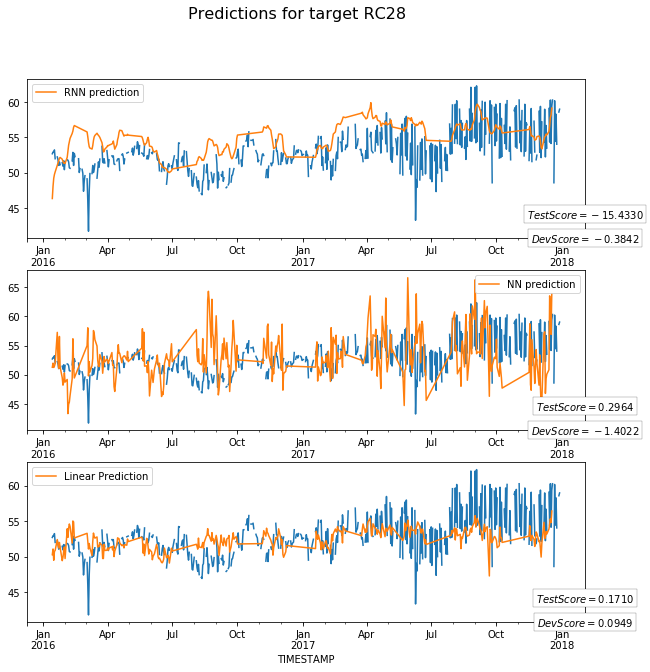
\includegraphics[width=0.9\columnwidth]{RC28.png}
\caption{Comparação dos 3 modelos na tarefa de regressão do índice RC28}
\end{figure}

\subsection{Segundo Ensaio}

Estudando os dados vemos que ouve um aumento repentino dos índices de dureza a
partir de 2016, e um ruído sensivelmente mais presente e com uma variância
maior. Várias tentativas foram feitas com diversos parâmetros de entrada e
nenhum conjunto destes ajuda a prever essa mudança brusca nos dados. Portanto
devemos concluir que ela é dada por fatores não presentes nos dados concedidos.
O primeiro ensaio foi realizado com os dados de treinamento sendo de 2008 a
2015, com o restante sendo nossos dados de validação. Uma performance melhor
possivelmente seria atingida se usarmos dados antes de 2016 para treinamento e
validação. \\  


Segue um plot da nova divisão dos dados entre treino/teste e validação para os índices que estamos modelando:


\begin{figure}[H]
\centering
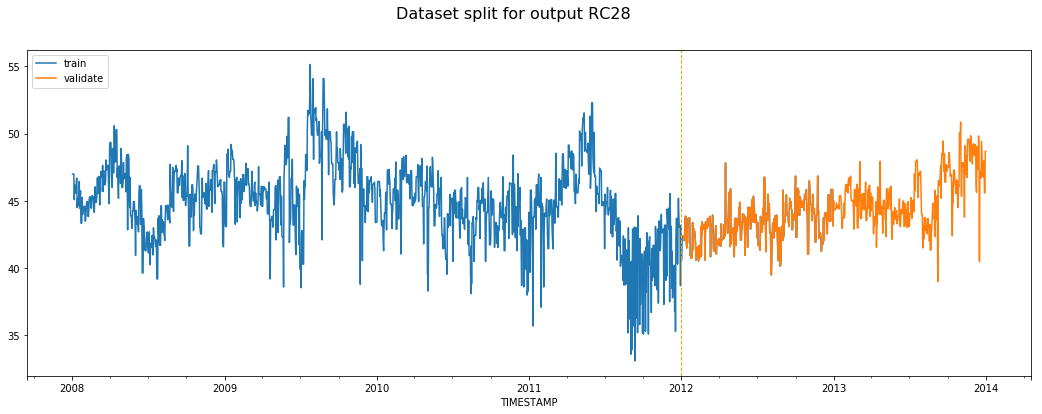
\includegraphics[width=0.9\columnwidth]{dataset_splitRC28.png}
\caption{Divisão do dataset para a saída RC28}
\end{figure}


Finalmente, seguem plots dos novos resultados, esses sendo reproduzidos apenas para o período inédito para os modelos, ou seja, o \textbf{dev set} de 2012 até 2014:

Primeiro, os modelos considerando os dados como não-sequenciais:

\begin{figure}[H]
\centering
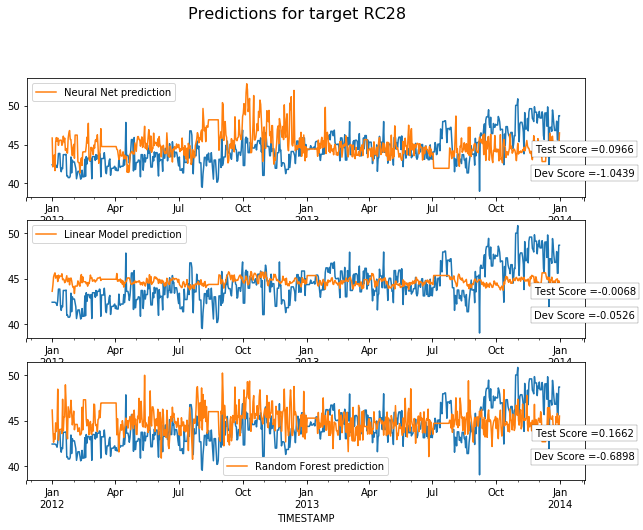
\includegraphics[width=0.9\columnwidth]{farinha_2008-2012-2014RC28.png}
\caption{Comparação dos 3 modelos não-sequenciais na tarefa de regressão do índice RC28}
\end{figure}


Agora, a performance da Rede Neural usando a técnica de Monte Carlo Dropout para inferência Bayesiana e cálculo de incerteza:


\begin{figure}[H]
\centering
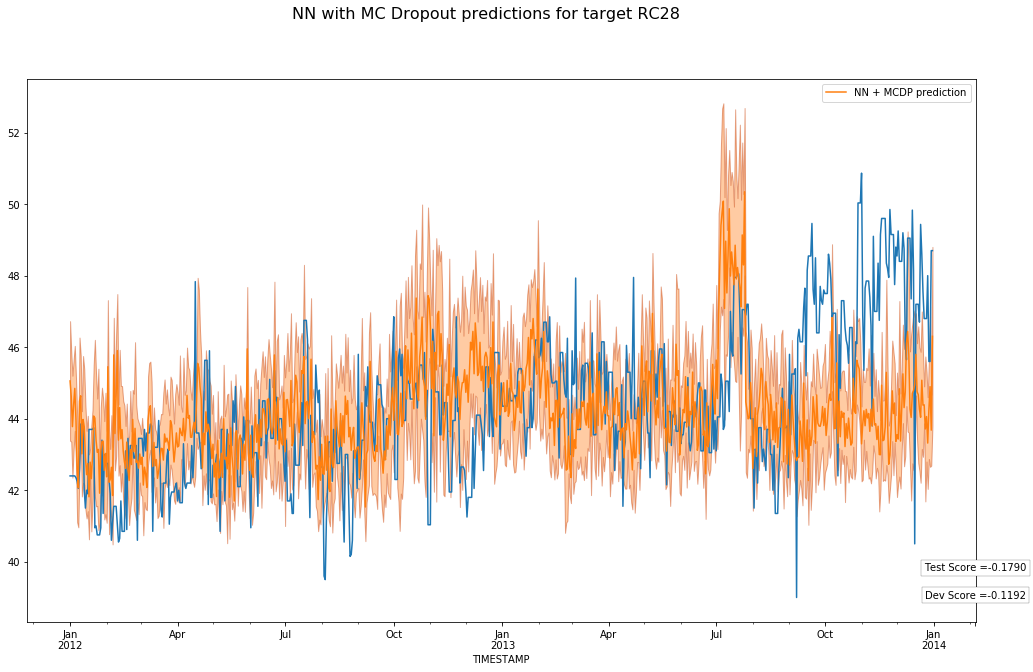
\includegraphics[width=1\columnwidth]{NNMCDP_2012-2014RC28.png}
\caption{Performance do modelo Rede Neural + MC Dropout para o índice RC28}
\end{figure}


É interessante notar que o modelo anterior com a sua capacidade de calcular incertezas, realiza uma boa tarefa de \say{cobrir} os dados reais com a sua incerteza prevista para os pontos de dados previstos. \\ 

Finalmente, temos o modelo de Rede Neural Recorrente, um modelo sequencial:

\begin{figure}[H]
\centering
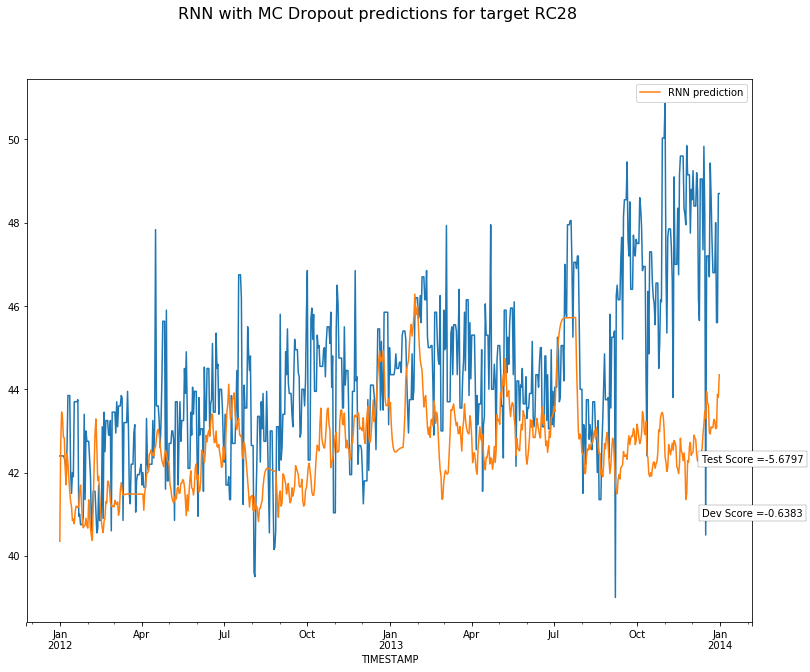
\includegraphics[width=0.9\columnwidth]{RNN_2012-2014RC28.png}
\caption{Performance do modelo RNN para o índice RC28}
\end{figure}


Dos resultados obtidos podemos perceber que a acurácia dos modelos aumenta sensivalmente para o índice RC28, isso se dá pelo fato que essa é uma medida na qual naturalmente está envolvido menos ruído e incerteza que as outras duas. Analisando os valores da métrica R2, os melhores modelos atingiram valores próximos de $0$.

%%% Local Variables:
%%% mode: latex
%%% TeX-master: "../quali"
%%% End:
